\documentclass{article}
\usepackage[utf8]{inputenc}
\usepackage[T1]{fontenc}
\usepackage{url}
\usepackage[margin=3cm]{geometry}
\usepackage{verbatim}
\usepackage[francais]{babel}
\newcommand\tab[1][1cm]{\hspace*{#1}}

\title{INFO-H303 - Projet - Partie 1}
\author{Wets Loukas, Alfaro Perez Victor, Muller Noëmie}


\begin{document}
\maketitle

\renewcommand{\abstractname}{}


\section{Modèle entité-association}
Insérer class-diagram ici (modélisant le projet et ses contraintes)

\iffalse
\begin{figure}[hb]
\begin{center}
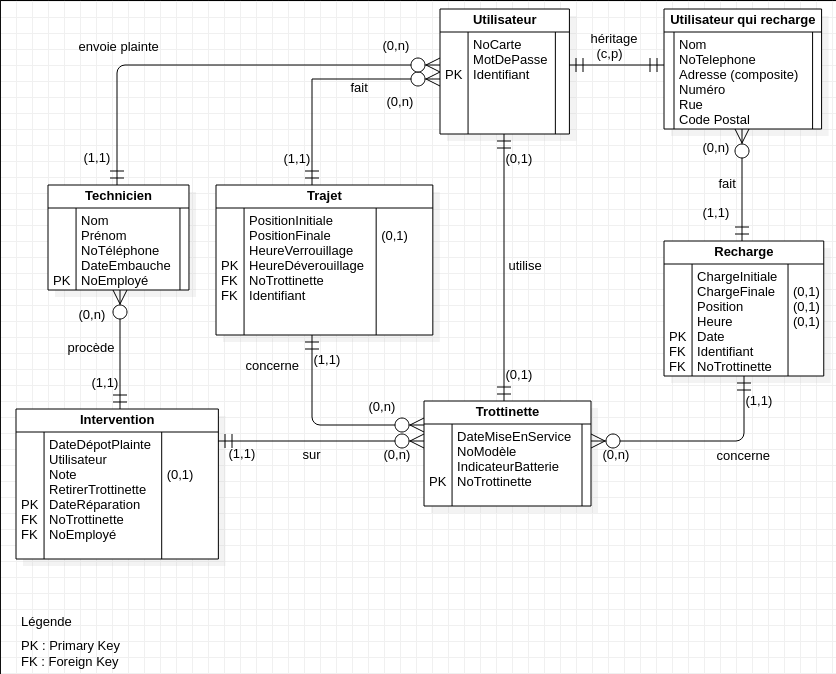
\includegraphics[scale=0.4]{image.png} 
\end{center}
\caption{Modèle entité-association}
\end{figure}
\fi 

\subsection*{Contraintes d'intégrité}

- La \textit{position initiale} de la \textit{trottinette} doit être à Bruxelles.

- La \textit{position finale} de la \textit{trottinette} doit être un numéro unique.

- L'\textit{indentifiant} de chaque \textit{trottinette}, de chaque \textit{utilisateur} et de chaque \textit{technicien} doit etre un numéro unique.

- Les \textit{trottinettes} ne doivent pas être tout à fait chargées pour être rechargées.

- La \textit{recharge} doit être éffectué entre 22h et 7h du matin.

- L'\textit{inspection} des trottinettes doit être effectué entre 22h et 7h du matin.

- La \textit{Date de réparation} doit être supérieur à la \textit{date de dépot} de la \textit{plainte}.

- La \textit{Date de mise en service} doit être inférieur à la \textit{date de dépot de painte}.

- Une \textit{trottinette} ne peut être utilisé que par un \textit{utilisateur} à la fois.

- Une \textit{trottinette} ne peut être réparé que par un \textit{technicien} à la fois.

- Une \textit{trottinette} ne peut être rechargé que par un \textit{utilisateur qui recharge} à la fois.

- Une \textit{trottinette} ne peut pas être \textit{utilisé} et être en même temps en train de \textit{chargé} ou en train d'être \textit{réparé}.

- La \textit{dateD'Intervention} doir être supérieur ou égale a la \textit{DateDeDépotDePlainte}.

-


\subsection*{Remarques}
Exprimer et justi??fier des hypothèses sur le modèle

\section{Modèle Relationnel}
Trottinette(\underline{N\textsuperscript{o}Trottinette}, DateMiseService, N\textsuperscript{o}Modèle, Etat, Identifiant)
\bigbreak
Utilisateur(\underline{Identifiant, MotDePasse}, N\textsuperscript{o}Carte)
\bigbreak
Technicien(\underline{N\textsuperscript{o}Employé}, Nom, Prenom, N\textsuperscript{o}Téléphone, DateEmbauche
\bigbreak
Trajet (\underline{HeureDeVerrouillage, N\textsuperscript{o}Trottinette, Identifiant}, HeurVerouillage, PositionInitiale)

\tab N\textsuperscript{o}Trottinette référence Trottinette.N\textsuperscript{o}Trottinette

\tab Identifiant référence Utilisateur.Identifiant
\bigbreak
UtilisateurQuiRecharge(\underline{Identifiant}, Nom, n\textsuperscript{o}Téléphone, AdresseRue, AdresseNumero, AdresseCommune, AdresseCodePostale)

\tab Identifiant référence Utilisateur.idnetifiant
\bigbreak
Recharge(\underline{Identifiant, N\textsuperscript{o}Trottinette, Date}, ChargeInitiale, ChargeFinale, Position, Heure)

\tab Identifiant référence UtilisateurQuiRecharge.Identifiant

\tab N\textsuperscript{o}Trottinette référence Trottinette.n\textsuperscript{o}Trottinette
 \bigbreak
 Intervention(\underline{N\textsuperscript{o}Trotinette, N\textsuperscript{o}Employe, DateReparation}, DateDéppotPlainte, Utilisateur, Note, RetirerTrottnette)
 
 \tab N\textsuperscript{o}Trottinette référence Trottinette.N\textsuperscript{o}Trottinette
 
\tab N\textsuperscript{o}Employé référence Technicien.N\textsuperscript{o}Trottinette
\bigbreak
TrottinetteUtilisateur(\underline{N\textsuperscript{o}Trottinette, Identifiant})

\tab N\textsuperscript{o}Trottinette référence Trottinette.N\textsuperscript{o}Trottinette

\tab Identifiant référence Utilisateur.Identifiant
\bigbreak
UtilisateurTechnicien(\underline{Identifiant, N\textsuperscript{o}Employé})

\tab Identifiant référence Utilisateru.Identifient

\tab N\textsuperscript{o}Employe référence Technicien.N\textsuperscript{o}Employé





\subsection*{Contraintes}
[...]

\subsection*{Remarques}
Justifier les choix de modélisation

Les deux modèles doivent servir de support aux requêtes suivantes :
R1 : La liste et la localisation des trottinettes actuellement disponibles.
R2 : La liste des utilisateurs ayant utilisé toutes les trottinettes qu'ils ont rechargées.
R3 : La trottinette ayant eeffectué la plus grande distance.
R4 : Les trottinettes ayant déjà fait l'objet d'au moins une dizaine de plaintes.
R5 : Les utilisateurs ayant déjà réalisé au moins 10 trajets avec pour chaque utilisateur concerné : la durée moyenne de ses trajets en trottinette, le nombre total de trajets réalisés, le montant total dépensé en trajets (sans prise en compte de l'argent gagné par les recharges éventuelles de trottinettes).





\end{document}
difftime|Ops\.factor|Ops\.numeric_version|Ops\.ordered|Ops\.POSIXt|options|order|ordered|outer|packageEvent|packageHasNamespace|packageStartupMessage|package_version|packBits|pairlist|parent\.env|parent\.frame|parse|parseNamespaceFile|paste|paste0|path\.expand|path\.package|pi|pipe|pmatch|pmax|pmax\.int|pmin|pmin\.int|polyroot|Position|pos\.to\.env|pretty|prettyNum|print|print\.AsIs|print\.by|print\.condition|print\.connection|print\.data\.frame|print\.Date|print\.difftime|print\.DLLInfo|print\.DLLInfoList|print\.DLLRegisteredRoutines|print\.factor|print\.function|print\.hexmode|print\.libraryIQR|print\.listof|print\.NativeRoutineList|print\.noquote|print\.numeric_version|print\.octmode|print\.packageInfo|print\.POSIXct|print\.POSIXlt|print\.proc_time|print\.restart|print\.rle|print\.simple\.list|print\.srcfile|print\.srcref|print\.summaryDefault|print\.summary\.table|print\.table|print\.warnings|prmatrix|proc\.time|prod|prop\.table|psigamma|pushBack|pushBackLength|q|qr|qr\.coef|qr\.fitted|qr\.Q|qr\.qty|qr\.qy|qr\.R|qr\.resid|qr\.solve|qr\.X|quarters|quarters\.Date|quarters\.POSIXt|quit|quote|range|rank|rapply|raw|rawConnection|rawConnectionValue|rawShift|rawToBits|rawToChar|rbind|rbind\.data\.frame|rcond|Re|readBin|readChar|read\.dcf|readline|readLines|readRDS|readRenviron|real|Recall|Reduce|regexec|regexpr|reg\.finalizer|registerS3method|registerS3methods|regmatches|remove|removeCConverter|removeTaskCallback|rep|rep\.Date|rep\.factor|rep\.int|replace|replicate|rep\.numeric_version|rep\.POSIXct|rep\.POSIXlt|require|requireNamespace|restartDescription|restartFormals|retracemem|rev|R\.home|rle|rm|RNGkind|RNGversion|round|round\.Date|round\.POSIXt|row|rowMeans|rownames|row\.names|row\.names\.data\.frame|rowsum|rowsum\.data\.frame|rowSums|R_system_version|R\.version|R\.Vera